\section{提案手法}
スマートフォン,もしくはタブレット端末にデータが送られてくる種類のドローンを対象としている.
まず通常飛行と同様にスマートフォンとドローンを任意の専用アプリケーションを用いて接続する.
その後,スマートフォンをPCに対して画面共有を行い,PCは共有された画面の映像を入力として,その映像に対し,Yolo v3を用いて物体検知を行い,その結果を描写した映像をPC上に表示する.
\begin{figure}[htbp]
  \begin{center}
    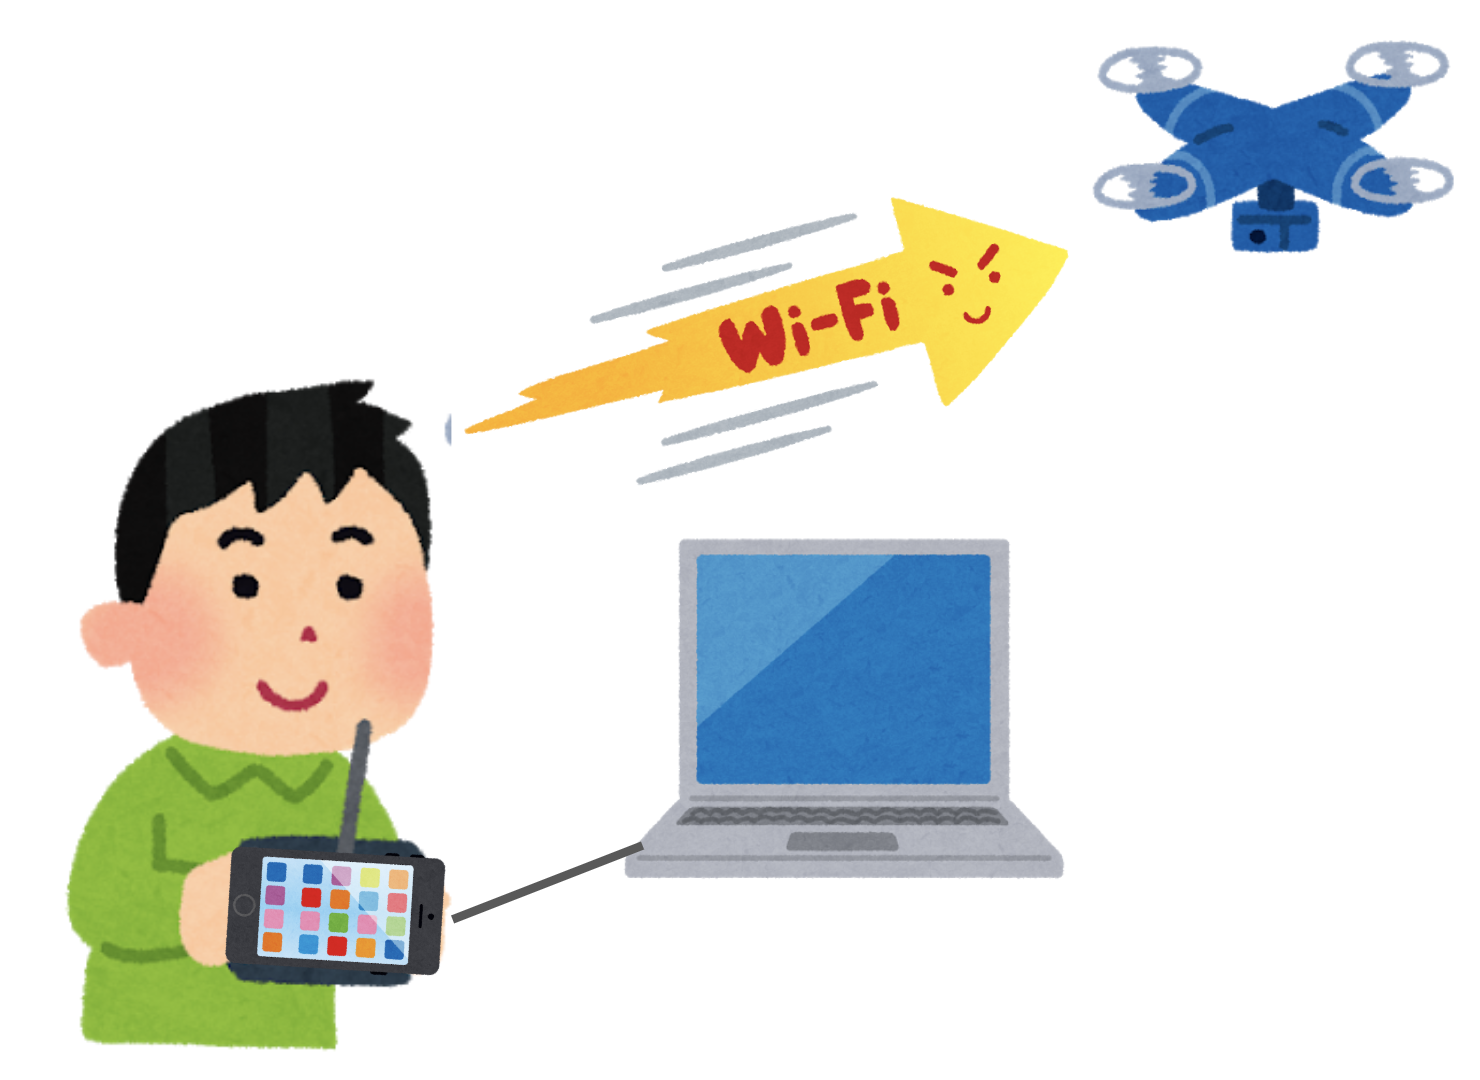
\includegraphics[clip,width=7.0cm]{img/sys-struct.png}
    \caption{構成図}
    \label{fig:struct}
  \end{center}
\end{figure}


\subsection{使用環境}
今回は以下の環境で開発を行った.
\begin{itemize}
  \item MacBookPro 2017 Model
  \item iPhone X
  \item QuickTime Player
  \item Python 3.6.8 |Anaconda|
  \item Yolo v3
\end{itemize}


